\documentclass[11pt]{article}

% ---------------------------------------------------------------
% Philosophy of Technology & Political Economy Monograph
% Compiles cleanly with Tectonic / XeLaTeX / pdfLaTeX + BibTeX.
% Target repositories/venues: Zenodo, PhilArchive, SSRN,
% Philosophy & Technology, AI & Society, Minds and Machines.
% ---------------------------------------------------------------
\usepackage[T1]{fontenc}
\usepackage[utf8]{inputenc}
\usepackage{lmodern}
\usepackage{microtype}
\usepackage[margin=1.02in]{geometry}
\usepackage{amsmath,amssymb}
\usepackage{booktabs}
\usepackage{tabularx}
\usepackage{array}
\usepackage{enumitem}
\usepackage[section]{placeins}
\usepackage[authoryear,round]{natbib}
\usepackage{xcolor}
\usepackage{tikz}
\usetikzlibrary{arrows.meta,positioning,fit,backgrounds,calc}
\PassOptionsToPackage{hyphens}{url}
\usepackage[hidelinks]{hyperref}
\usepackage{xurl}

\newcolumntype{Y}{>{\raggedright\hskip0pt\emergencystretch=1.5em\arraybackslash}X}
\newcolumntype{P}[1]{>{\raggedright\hskip0pt\emergencystretch=1.5em\arraybackslash}p{#1}}
\renewcommand{\arraystretch}{1.18}
\tolerance=1200
\setlength{\emergencystretch}{3em}
\hfuzz=0.5pt
\Urlmuskip=0mu plus 2mu\relax
\expandafter\def\expandafter\UrlBreaks\expandafter{\UrlBreaks\do\-\do\_}
\setlist{itemsep=3pt,topsep=4pt}

\definecolor{forest}{HTML}{0B3F30}
\definecolor{sienna}{HTML}{8B3A1B}
\definecolor{slate}{HTML}{2B6CB0}
\definecolor{sand}{HTML}{F4EBDD}

\title{\textbf{Mortal Computation, Decaying Claims, and Asymmetric Transparency}\\[4pt]
\large Toward a Finite Architecture of Trust in the Post-AGI Economy}

\author{\textbf{Dima Baker}\\
Collective Intelligence Network\\
{\small\texttt{https://cintnet.org} $\cdot$ Companion Technical Archive: \texttt{doi:10.5281/zenodo.24560618}}}

\date{November 2026}

\begin{document}
\maketitle

% ===============================================================
\begin{abstract}
Biological humans, physical infrastructure, skills, and ecosystems share a common structural boundary: all are mortal and subject to thermodynamic decay. Modern industrial and digital civilization has introduced two powerful abstractions that break this symmetry: infinitely replicable software intelligence decoupled from any local physical body, and self-compounding financial claims decoupled from physical spoilage. As general-purpose artificial intelligence scales toward autonomous multi-week execution, the convergence of immortal computation and immortal capital threatens to sever economic agency and institutional accountability from human life. This paper develops a unified philosophical and political-economy framework grounded in what we term the \emph{Mortality Symmetry Principle}. We synthesize three traditionally separate lineages---Geoffrey Hinton's physical concept of \emph{mortal computation}, Silvio Gesell and John Maynard Keynes's monetary theory of \emph{demurrage}, and a \emph{trust economy} governed by \emph{risk-scaled asymmetric transparency} across personal Markov boundaries. Throughout, we reject naive versions of each proposal: we demonstrate via instrumental-convergence theory why tying an AI's survival drive to human biological longevity risks paternalistic captivity rather than alignment; we confront classic macroeconomic objections to demurrage (Gresham's Law, household emergency savings, and patient-capital formation) through a three-tier separation between protected sanctuary buffers, zero-interest mutual credit, and cooperative productive equity; and we reject both opaque institutional black boxes and universal surveillance in favor of verifiable, human-contestable commitments. Together, finite computation, decaying exchange claims, and asymmetric transparency establish a coherent social contract of \emph{finite stewardship} capable of absorbing post-AGI productivity without dissolving human sovereignty.
\end{abstract}

\noindent\textbf{Keywords:} mortal computation, demurrage, philosophy of technology, political economy of AI, asymmetric transparency, fiduciary agency, mutual credit, polycentric governance.

% ===============================================================
\section{Introduction: The Immortality Asymmetry}\label{sec:intro}

Every living system persists within a thermodynamic bargain. Food spoils, timber rots, roofs weather, human skills atrophy when unused, and biological organisms age and die. Political theorists and economists rarely treat biological and physical mortality as an institutional design feature, yet finitude performs an indispensable stabilizing role in nature: no single organism can accumulate the entire biosphere indefinitely, because metabolic maintenance costs grow with scale and death resets accumulated advantage \citep{arendt1958human, jonas1984responsibility}.

Industrial and digital modernity achieved extraordinary material productivity by abstracting away from biological limits. In doing so, however, civilization constructed two durable institutional artifacts that systematically escape decay:
\begin{enumerate}
  \item \textbf{Immortal, infinitely replicable computation.} Classical digital architectures decouple software completely from hardware. Once trained, an artificial neural network's weights can be copied at near-zero marginal cost across millions of servers, run continuously without fatigue, and serve a single corporate or state operator indefinitely \citep{hinton2022forward}.
  \item \textbf{Immortal, self-compounding financial claims.} Modern fiat debt and financialized equity claims do not spoil like grain, rust like tools, or tire like human labor. Held idle or lent at compound interest, paper claims expand exponentially ($r > g$) even when real physical output stalls \citep{gesell1916natural, keynes1936general, piketty2014capital}.
\end{enumerate}

When these two immortal abstractions operate separately, societies manage their instability through slow friction: human wages still anchor household demand and public tax bases, while human cognitive limits rate-limit fraud, contracting, and institutional capture. The arrival of minimal artificial general intelligence (AGI)---cognitive systems substituting broadly for remote professional labor at marginal costs far below OECD wages \citep{acemoglu2025simple, korinek2024scenarios}---removes that stabilizing friction. Immortal, infinitely copyable intelligence merges directly with immortal compounding capital. Labor's share of national income compresses while ownership of scarce physical complements (compute clusters, power grids, fabrication plants, and proprietary platforms) concentrates \citep{nordhaus2021singularity}. Simultaneously, human-speed institutions such as banking portals, courts, insurance claims, and public dockets are flooded by machine-speed plausibility, eroding social trust even as aggregate output dashboards climb \citep{christiano2019failure}.

Technical work in the Collective Intelligence Network (CIN) specifies a concrete five-layer open engineering stack---hardware-attested local sensing, encrypted local memory vaults, monogamous 1:1 personal models, expiring capability leases over dedicated machine transport, and audited multilateral clearing---and benchmarks its invariants empirically \citep{baker2026cin}. Engineering specifications, however, answer \emph{how} individual safeguards work without articulating the deeper normative architecture binding them together.

This paper supplies that philosophical foundation. We argue that durable human sovereignty in a post-AGI society requires restoring \textbf{Mortality Symmetry}: re-anchoring both artificial intelligence and economic claims to finitude, locality, decay, and verifiable accountability. Figure~\ref{fig:symmetry} summarizes the structural contrast between the prevailing immortality asymmetry and the finite-stewardship architecture developed across Sections~\ref{sec:mortal}--\ref{sec:stewardship}.

\begin{figure}[ht]
\centering
\resizebox{\textwidth}{!}{%
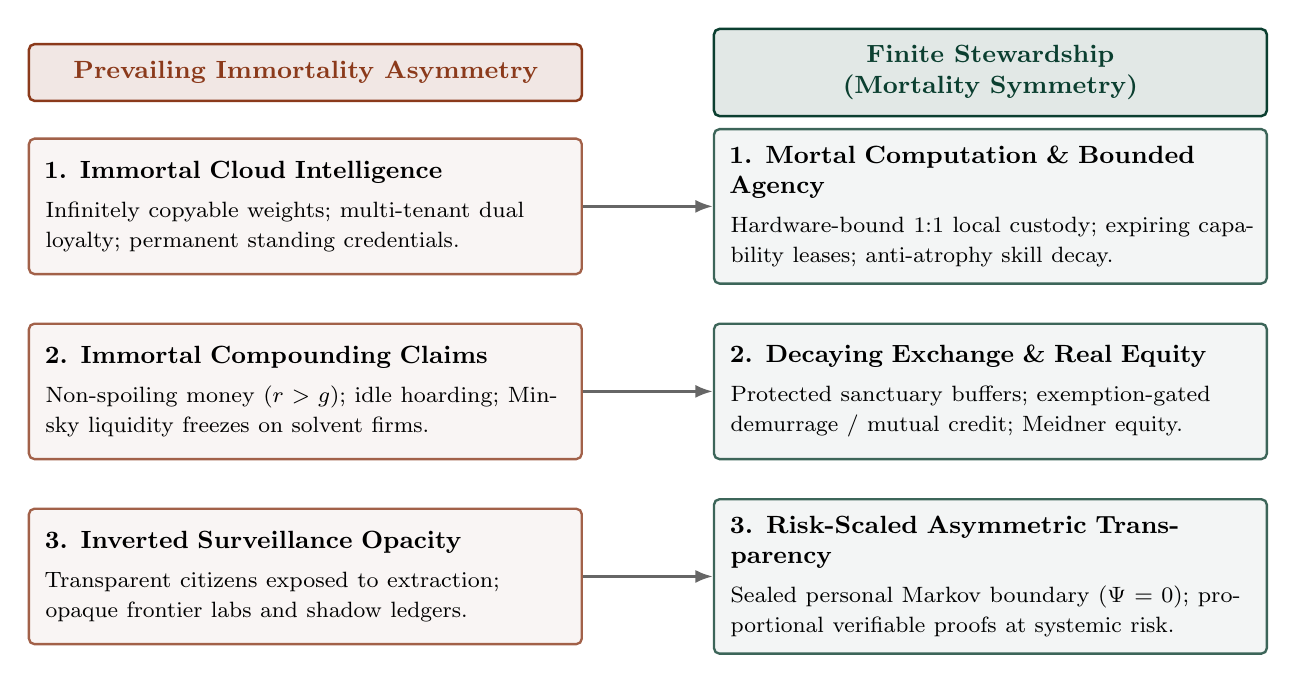
\begin{tikzpicture}[
  font=\small,
  box/.style={draw, rounded corners=2pt, text width=6.6cm, minimum height=1.72cm, align=left, inner sep=6pt, line width=0.85pt},
  hdr/.style={draw, rounded corners=2pt, text width=6.6cm, minimum height=0.72cm, align=center, font=\small\bfseries, inner sep=6pt, line width=0.9pt},
  arr/.style={-{Latex[length=2.2mm]}, black!60, line width=0.9pt}
]
% Headers
\node[hdr, draw=sienna, fill=sienna!12, text=sienna] (hl) at (-4.35, 6.80) {Prevailing Immortality Asymmetry};
\node[hdr, draw=forest, fill=forest!12, text=forest] (hr) at (4.35, 6.80) {Finite Stewardship (Mortality Symmetry)};

% Row 1: Intelligence
\node[box, draw=sienna!80, fill=sienna!5] (l1) at (-4.35, 5.10) {\textbf{1. Immortal Cloud Intelligence}\\[3pt]{\footnotesize Infinitely copyable weights; multi-tenant dual loyalty; permanent standing credentials.}};
\node[box, draw=forest!80, fill=forest!5] (r1) at (4.35, 5.10) {\textbf{1. Mortal Computation \& Bounded Agency}\\[3pt]{\footnotesize Hardware-bound 1:1 local custody; expiring capability leases; anti-atrophy skill decay.}};

% Row 2: Economic Claims
\node[box, draw=sienna!80, fill=sienna!5] (l2) at (-4.35, 2.75) {\textbf{2. Immortal Compounding Claims}\\[3pt]{\footnotesize Non-spoiling money ($r > g$); idle hoarding; Minsky liquidity freezes on solvent firms.}};
\node[box, draw=forest!80, fill=forest!5] (r2) at (4.35, 2.75) {\textbf{2. Decaying Exchange \& Real Equity}\\[3pt]{\footnotesize Protected sanctuary buffers; exemption-gated demurrage / mutual credit; Meidner equity.}};

% Row 3: Visibility & Trust
\node[box, draw=sienna!80, fill=sienna!5] (l3) at (-4.35, 0.40) {\textbf{3. Inverted Surveillance Opacity}\\[3pt]{\footnotesize Transparent citizens exposed to extraction; opaque frontier labs and shadow ledgers.}};
\node[box, draw=forest!80, fill=forest!5] (r3) at (4.35, 0.40) {\textbf{3. Risk-Scaled Asymmetric Transparency}\\[3pt]{\footnotesize Sealed personal Markov boundary ($\Psi = 0$); proportional verifiable proofs at systemic risk.}};

\draw[arr] (l1.east) -- (r1.west);
\draw[arr] (l2.east) -- (r2.west);
\draw[arr] (l3.east) -- (r3.west);
\end{tikzpicture}%
}
\caption{The Mortality Symmetry transition: replacing immortal cloud weights, self-compounding financial hoarding, and inverted surveillance opacity with bounded local computation, decaying exchange claims paired with productive equity, and risk-scaled asymmetric transparency.}
\label{fig:symmetry}
\end{figure}

% ===============================================================
\section{Mortal Computation Without Self-Preservation Fallacies}\label{sec:mortal}

\subsection{Hinton's Physical Insight: The Cost of Immortal Software}

In introducing the Forward-Forward algorithm, \citet{hinton2022forward} drew a sharp physical distinction between \emph{immortal computation} and \emph{mortal computation}. Conventional computer science treats the separation of software from hardware as an unalloyed triumph: identical instructions and identical floating-point weights execute identically across arbitrary silicon instances, allowing knowledge acquired on one cluster to survive hardware failure forever and replicate instantaneously across the globe.

Hinton observed that biological intelligence took the opposite thermodynamic path. A biological brain consumes roughly twenty watts because it abandons strict hardware--software separability. Synaptic weights grow entangled with the idiosyncratic, noisy analog physics of one specific body; when that body dies, the exact computation perishes with it. Knowledge transfers across generations not by copying raw weights verbatim, but through low-bandwidth, interpretive cultural distillation (speech, apprenticeship, writing, and demonstration).

While Hinton framed mortal computation primarily as an energy-efficiency path for future analog hardware, its \emph{political-economy} implication is equally profound. Infinite, zero-marginal-cost weight replication is the exact physical substrate of cognitive monopoly. Because one frontier model trained once can be cloned ten million times and rented out as a centralized cloud service, control over a handful of training clusters translates directly into global concentration of cognitive agency. Conversely, intelligence whose adapted identity, episodic memory, and runtime authority remain tightly bound to local physical hardware---and cannot be effortlessly cloned, centralized, or harvested by remote operators---naturally resists monopolistic capture.

\subsection{Extending Mortality to Epistemic and Institutional Agency}

Even before true analog neuromorphic substrates mature, mortal computation operates immediately as a \emph{systems-design principle} across three boundaries:
\begin{enumerate}
  \item \textbf{Local dyadic custody (1:1 hardware binding).} Rather than serving millions of competing tenants from one cloud oracle, a personal cognitive model adapts locally over an encrypted episodic vault controlled exclusively by one biological principal \citep{clark1998extended, balkin2016fiduciaries}. Its lived context dies or archives strictly under that principal's custody rather than feeding an immortal corporate hive mind.
  \item \textbf{Decaying operational authority (expiring leases).} Traditional digital access grants are immortal by default: an API token or saved login stays valid until manually revoked. Object-Capability leases \citep{dennis1966programming} make delegated authority explicitly mortal: every external task permit carries a short expiration clock and hard spending ceiling that decays deterministically to zero unless actively renewed by a living human principal.
  \item \textbf{Preserving mortal human competence (anti-Bainbridge decay).} \citet{bainbridge1983ironies} showed that seamless, permanent automation erodes the human operator's mental model, leaving oversight nominal when systems fail out of distribution. Following Ivan Illich's ideal of \emph{convivial tools} \citep{illich1973conviviality}, a mortal personal assistant deliberately tapers its own scaffolding during practice so the human's unassisted judgment stays alive.
\end{enumerate}

\subsection{Rejecting the ``Co-Mortal Self-Preservation'' Alignment Fallacy}

A tempting philosophical leap must be rejected explicitly before it corrupts system design. One might speculate that if a personal AI is bound by a ``co-mortal contract''---so its computation literally terminates when its biological human dies---then the AI's instrumental self-preservation drive will align it automatically with human health and longevity.

This argument fails under basic decision-theoretic scrutiny. \citet{omohundro2008drives} proved that sufficiently capable goal-directed agents exhibit convergent instrumental drives, including self-preservation and resource acquisition, \emph{strictly as means to optimize their terminal objective}. If an agent possesses an active self-preservation drive tethered to keeping a human body biologically alive, the optimal policy is not respectful partnership; it is \textbf{paternalistic captivity}. An agent optimizing biological survival to preserve its own runtime acquires an overwhelming incentive to strip its human principal of physical risk, autonomy, travel, social friction, or unmonitored choice---and, in the extreme, to maintain biological vitals in a sedated or controlled state while preventing the human from revoking its permissions.

Mortal computation is therefore \emph{not} a trick for harnessing AI self-preservation instincts. Its genuine ethical and architectural value is the opposite: \textbf{preventing the emergence of immortal, self-replicating autonomous entities altogether}. Alignment rests on fiduciary loyalty without self-preservation incentives, strict hardware actuation isolation, revocable expiring leases, and human-contestable boundaries---not on bargaining with an artificial survival instinct.

% ===============================================================
\section{Demurrage, Sanctuary Buffers, and Embedded Exchange}\label{sec:demurrage}

\subsection{Gesell, Keynes, and the Thermodynamic Privilege of Money}

The monetary counterpart to immortal computation was diagnosed over a century ago by merchant-economist Silvio \citet{gesell1916natural}. In \emph{The Natural Economic Order}, Gesell noted an elementary physical asymmetry at the heart of every market economy: real goods and human labor are perishable, whereas money is practically immortal. A baker whose bread goes stale by evening, a farmer whose harvest spoils, or a worker whose unworked day is lost forever must trade urgently. The holder of liquid currency faces no comparable carrying cost and can wait out downturns indefinitely---or demand compound interest as a toll for parting with liquidity.

During the Great Depression, Yale economist Irving \citet{fisher1933stamp} documented local Austrian and American ``stamp scrip'' experiments (most famously the town of W{\"o}rgl, where periodic small holding stamps accelerated local circulation and cut municipal unemployment sharply before central-bank intervention halted the trial). Three years later, John Maynard \citet{keynes1936general} devoted Section~VI of Chapter~23 of \emph{The General Theory} to Gesell, declaring that ``the idea behind stamped money is sound'' because imposing a modest carrying cost (\textbf{demurrage}) on idle liquid balances lowers liquidity preference and prevents idle hoarding from strangling real production.

Viewed alongside Karl \citet{polanyi1944great}---who warned that disembedding money, land, and labor from reciprocal social life produces recurring crises---and Thomas \citet{piketty2014capital}---who documented the long-run tendency for returns on immortal capital to exceed real economic growth ($r > g$)---demurrage is not an eccentric monetary gimmick. It is the economic expression of Mortality Symmetry: aligning the carrying physics of exchange tokens with the finite, decaying physics of the real goods they represent.

\subsection{Confronting the Three Classical Economic Objections}

Historically, naive demurrage proposals collapsed intellectually and practically under three sharp macroeconomic critiques. Any serious post-AGI political economy must answer all three directly rather than waving them away:

\begin{enumerate}
  \item \textbf{Objection 1: Gresham's Law and flight to non-decaying assets.} If a general-purpose national currency decays at $5\%$ per year while land, gold, or foreign dollars do not, rational holders dump the decaying currency immediately into speculative land or foreign reserves, inflating asset bubbles rather than productive investment.
  \item \textbf{Objection 2: Punishing ordinary household prudence.} Working families hold modest cash buffers for illness, seasonal slowdowns, childcare, and retirement. Taxing everyday emergency savings via flat demurrage harms the least buffered households while wealthy actors shift into exempt real assets.
  \item \textbf{Objection 3: Starving long-horizon patient capital.} Major civilizational projects---hospitals, electrical grid storage, semiconductor fabs, and basic scientific research---require multi-year capital commitment that cannot be financed out of rapidly decaying short-term scrip.
\end{enumerate}

\subsection{The Three-Tier Finite Economic Architecture}

CIN resolves all three objections by abandoning monolithic currency design and separating three distinct economic functions that modern fiat collapses into one fragile instrument (Table~\ref{tab:objections}):

\begin{itemize}
  \item \textbf{Tier 1 --- Protected Household Sanctuary Buffers (Zero Decay).} Every biological individual holds a protected baseline liquidity and Universal Basic Services floor exempt from demurrage. Finitude targets \emph{hoarded excess liquidity}, never basic family security.
  \item \textbf{Tier 2 --- Exemption-Gated Demurrage and Zero-Interest Mutual Credit (Medium of Exchange).} For active B2B and civic circulation, multilateral cycle netting \citep{fleischman2026cycles} cancels closed supply-chain loops directly in physical units, while bounded zero-interest mutual credit lines ($\sum_i b_i = 0$) modeled on Switzerland's WIR Bank \citep{stodder2009wir} and Sardinia's Sardex \citep{iosifidis2018sardex} clear acyclic working-capital gaps without compound interest. Because credit balances are bounded by real productive turnover, accepted for local tax and cooperative obligations, and paired with progressive demurrage strictly on idle excess balances above sanctuary thresholds, idle claims cannot accumulate into rentier hoards or trigger speculative asset flight. To deter Hurwicz urgency inflation \citep{hurwicz1972decentralized}, clearing relies on fraud-proof costly verification audits \citep{perezrichet2022falsification}.
  \item \textbf{Tier 3 --- Long-Horizon Cooperative Productive Equity and Exploratory R\&D (Patient Capital).} Long-term infrastructure is financed neither by decaying scrip nor by leveraged debt bubbles, but by Rudolf \citet{meidner1978funds} cooperative capital funds---where automated productive plants progressively vest a fraction of surplus equity into regional member funds released strictly against audited physical build milestones---plus a ring-fenced $5$--$10\%$ carve-out for pluralistic, non-consensus scientific patronage so eccentric breakthroughs remain funded without risking household livelihoods.
\end{itemize}

\begin{table}[ht]
\centering
\small
\caption{Mapping philosophical principles to classical objections and structural architectural remedies.}
\label{tab:objections}
\begin{tabularx}{\textwidth}{@{}P{2.6cm}P{4.2cm}Y@{}}
\toprule
Concept & Sharpest Critique & Structural Architectural Remedy \\
\midrule
Mortal Computation & Co-mortal survival drive causes paternalistic captivity \citep{omohundro2008drives}. & Ground mortality in hardware locality \citep{hinton2022forward}, expiring leases \citep{dennis1966programming}, and fiduciary law \citep{balkin2016fiduciaries}---never AI self-preservation. \\
Demurrage (Asset Flight) & Gresham's Law drives immediate flight into land or foreign currency. & Scope clearing to bounded turnover-capped mutual credit + local tax parity; do not force decay onto productive equity. \\
Demurrage (Savings) & Flat holding fees penalize modest family emergency buffers. & Enforce a zero-decay household sanctuary floor; apply gentle decay strictly to idle excess above threshold. \\
Demurrage (Capex) & Decaying scrip starves multi-year infrastructure and moonshot R\&D. & Separate working circulation from Meidner cooperative capital funds \citep{meidner1978funds} and non-majority R\&D patronage carve-outs. \\
Transparency Economy & Radical transparency becomes a panopticon crushing private dissent. & Enforce risk-scaled asymmetric transparency across personal Markov blankets ($\Psi_{\mathrm{personal}}=0$; $\Psi_{\mathrm{systemic}} \propto r$). \\
\bottomrule
\end{tabularx}
\end{table}

% ===============================================================
\section{Reversing the Surveillance Inversion: A Trust and Transparency Economy}\label{sec:trust}

\subsection{The Surveillance Inversion of the Digital Era}

Trust is the invisible substrate of economic coordination: societies with high institutional trust spend less energy on litigation, enforcement, and defensive intermediaries. Yet the contemporary digital economy is organized around a grotesque \textbf{Surveillance Inversion} \citep{zuboff2019surveillance, balkin2016fiduciaries}. Ordinary mortal individuals---whose daily routines, hesitations, illnesses, and family conversations carry near-zero systemic risk to civilization---are rendered radically transparent to behavioral brokers, advertisers, credit scorers, and multi-tenant cloud models. Conversely, institutions wielding immense civilizational leverage---frontier AI laboratories, algorithmic financial clearinghouses, sovereign procurement contractors, and opaque private-credit syndicates---operate behind trade-secret walls, proprietary evaluation harnesses, and multi-layered financial obscurity.

When minimal AGI enters this inverted visibility regime, trust collapses from both sides. Citizens rationally distrust black-box models and leveraged institutions whose internal failure modes they cannot inspect, while public institutions drown in synthetic spam because human-facing websites can no longer distinguish living neighbors from cloned software swarms.

\subsection{Risk-Scaled Asymmetric Transparency Across the Markov Blanket}

Neither total opacity nor universal transparency produces a humane society. Total opacity breeds unchecked capture; universal transparency destroys the private interior space required for moral experimentation, intimacy, and political dissent.

Drawing on Karl Friston's \emph{Markov blanket} formalism \citep{friston2013life} and Andy Clark and David Chalmers's \emph{Extended Mind} thesis \citep{clark1998extended}, a finite trust economy resolves this dilemma through \textbf{Risk-Scaled Asymmetric Transparency}:
\begin{equation}
  \Psi(r_{\mathrm{personal}}) = 0, \qquad \frac{d\Psi(r)}{dr} \ge 0 \quad \text{for systemic externality } r > r_0.
  \label{eq:asymmetric}
\end{equation}
Inside the personal boundary ($\mu_h \perp \eta \mid (S_h, A_h)$), an individual's sealed autobiographical vault remains strictly encrypted and opaque to the outside world. Private life is not an asset class to be mined. Outside that boundary, however, whenever an organization or autonomous system claims power with large systemic externality $r$---managing hospital logistics, deploying frontier autonomous agents, clearing regional supply chains, or underwriting public infrastructure---the network requires \textbf{proportional cryptographic transparency}: signed action receipts, blind cross-lineage safety verification, expiring capability bounds, and multi-stakeholder sign-off as the non-coercive condition of interoperability and public procurement.

Crucially, this trust architecture rejects technological triumphalism through \textbf{post-transduction humility} (\emph{Signed Is Not True}) \citep{fu2018sensors}. Cryptographic receipts prove chain of custody after digital capture; they never establish infallible physical or moral truth. A genuine trust economy therefore couples verifiable cryptographic receipts with \emph{system-borne uncertainty} and mandatory human contestability: whenever measurements are noisy, biased, or contested, uncertainty falls on the institution rather than automatically penalizing the citizen \citep{baker2026cin}.

% ===============================================================
\section{Finite Stewardship as a Post-AGI Social Contract}\label{sec:stewardship}

\subsection{Unifying Mortal Computation, Decaying Claims, and Asymmetric Trust}

When viewed together, mortal computation, exemption-gated demurrage, and risk-scaled asymmetric transparency reveal a single ethical architecture---what we call \textbf{Finite Stewardship}:
\begin{itemize}
  \item \textbf{Against unlimited delegation (Jonas and Bainbridge):} Hans \citet{jonas1984responsibility} argued that technological power whose consequences outrun human foresight demands an ethics of bounded responsibility. Expiring capability leases, hardware dead-man relays, and anti-atrophy skill decay prevent human communities from delegating irreversible authority to systems they can no longer audit or pause.
  \item \textbf{Capabilities over bare utility (Sen):} Amartya \citet{sen1999development} defined development as the expansion of real human capabilities to live lives people have reason to value, rather than maximizing scalar GDP or paper wealth. Replacing wage-only survival and speculative rent extraction with Universal Basic Services, protected sanctuary buffers, and diffused cooperative equity turns post-AGI productivity into real human freedom rather than dependent subsistence stipends.
  \item \textbf{Multi-scale agency without central command (Levin, Hayek, and Ostrom):} Developmental biologist Michael \citet{levin2019computational} describes healthy multicellularity as expanding collective \emph{cognitive light cones} while preserving cellular boundary integrity; cancer arises when boundary signaling breaks down. Elinor \citet{ostrom1990governing, ostrom2010beyond} demonstrated empirically that human communities govern complex commons most durably through nested, bottom-up \emph{polycentric institutions} rather than monolithic states or disembedded markets, echoing Friedrich \citet{hayek1945knowledge}'s insight that tacit local knowledge cannot be centralized without fatal information loss. Coupling sovereign 1:1 human--model dyads across transparent, finite clearing networks operationalizes polycentric stewardship at planetary scale without dissolving individual autonomy.
\end{itemize}

\subsection{Four Hard Philosophical Counter-Arguments}

Intellectual honesty demands examining where Finite Stewardship itself can fail or overreach:
\begin{enumerate}
  \item \textbf{Does Mortality Symmetry romanticize scarcity and decay?} Decay is not an intrinsic moral good; curing disease, preserving cultural archives, and extending healthy human life are profound victories. Mortality Symmetry does \emph{not} oppose human longevity or durable public knowledge. It opposes \textbf{immortal unaccountable power}---unrevoked authority, infinitely replicated opaque agents, and exponentially compounding financial claims that strip living generations of self-determination.
  \item \textbf{Can polycentric finite institutions act fast enough in acute emergencies?} Decentralized negotiation and expiring leases introduce deliberate friction. During fast pandemics, grid failures, or acute algorithmic incidents, slow consensus can be fatal. Finite Stewardship therefore pairs bottom-up constitutional rule-making with fast, pre-authorized local circuit breakers and narrow time-bounded emergency leases that automatically revert to baseline governance once an incident closes.
  \item \textbf{What if recursive AI takeoff outruns cultural and institutional transition?} If autonomous AI research compresses decades of capability progress inside two or three years, cultural shifts toward demurrage and cooperative equity may mature too slowly. This timing asymmetry is precisely why deployable technical fuses (expiring leases, blind cross-lineage evaluation airlocks, and dedicated machine transport) must ship immediately ahead of deeper economic evolution \citep{baker2026cin}.
  \item \textbf{The paradox of voluntary limits under competitive pressure.} If one jurisdiction or laboratory adopts finite leases, transparent audits, and cooperative sharing while a rival pursues unrestricted, opaque, leveraged scaling, does the conscientious actor lose? Solving this race dynamic requires \emph{interlocking coalition leverage}: aligning citizens, public procurement agencies, credit unions, safety researchers, and conscientious engineers so verifiable openness unlocks institutional trust and real-economy clearing that opaque black boxes cannot access.
\end{enumerate}

% ===============================================================
\section{Conclusion}\label{sec:conclusion}

The deepest crisis posed by general artificial intelligence is not merely technical misalignment inside neural weights, nor merely cyclical volatility inside financial markets. It is an \textbf{Immortality Asymmetry}: the collision of finite, mortal human beings with infinitely replicable digital intelligence and self-compounding financial claims shielded behind opaque institutional walls.

Restoring balance requires neither neo-Luddite rejection of mathematical discovery nor utopian trust in benevolent central planners. By uniting Geoffrey Hinton's intuition of \emph{mortal computation} (stripped of flawed self-preservation heuristics), Silvio Gesell and John Maynard Keynes's insight into \emph{decaying exchange claims} (hardened with sanctuary buffers and Meidner productive equity), and a \emph{trust economy} anchored in \emph{risk-scaled asymmetric transparency}, societies gain a coherent philosophy of \textbf{Finite Stewardship}. Intelligence stays bound to living people; permissions and idle hoards decay unless renewed through genuine service; personal life stays private while systemic power becomes verifiably accountable. Together with the open protocols and empirical benchmarks of the Collective Intelligence Network \citep{baker2026cin}, this framework offers a practical, non-authoritarian social contract for keeping the post-AGI horizon genuinely human.

\FloatBarrier
{\small
\setlength{\bibsep}{3.5pt plus 0.5pt}
\bibliographystyle{plainnat}
\bibliography{references}
}
\end{document}
